\section[Contexte des langages dédiés s'appliquant aux ordonnanceurs d'E/S sous Linux (A CHANGER)]{Contexte des langages dédiés s'appliquant aux or-donnanceurs d'E/S sous Linux (A CHANGER)}
\label{context}

\subsection{Les planificateurs d'E/S}

Dans leur fonctionnement, les ordonnanceurs de lecture (sortie) et d'écriture 
(entrée) tentent d'améliorer le débit en réorganisant l'accès aux requêtes dans 
un ordre linéaire basé sur les adresses logiques des données sur le disque, en 
essayant de les fusionner. Bien que cela puisse augmenter le débit global, 
certaines requêtes d'E/S peuvent attendre trop longtemps, provoquant des 
problèmes de latence et des fois de famine. Les planificateurs d'E/S tentent 
d'équilibrer le besoin d'un débit élevé tout en essayant de partager 
équitablement les requêtes d'E/S entre les processus.

Différentes approches ont été adoptées pour divers planificateurs d'E/S et 
chacun a ses propres forces et faiblesses et de manière générale, il n'y a pas 
de planificateur d'E/S par défaut parfait pour toute la gamme de requêtes d'E/S 
qu'un système peut rencontrer. 

\subsection{État de l'art}

Historiquement, les premiers algorithmes d'ordonnancement qui ont été 
développés se sont basés sur la structure interne des disques durs de l'époque, 
que l'on retrouve aujourd'hui encore dans beaucoup d'ordinateur. Cette 
structure organisée par secteurs de données sur plateaux était lue par une tête 
de lecture unique, limitant ainsi les actions possibles sur le disque à une 
seule écriture ou une seule lecture à la fois. Les algorithmes de l'époque ont 
donc étaient développés en conséquence, et sont devenus au fur et à mesure du 
temps obsolètes. La sortie de nouvelles technologies à la mémoire flash, comme 
les disques SSD (Solid-State Drive) ont offert la possibilité de pouvoir 
effectuer plusieurs lectures et plusieurs écritures de manière simultanée. Ces 
nouvelles technologies ont donc donnée naissance à de nouveaux algorithmes, 
comme BFQ en 2003, ou Kyber, développé en 2017 par Facebook.

Aujourd'hui dans Linux il existe plusieurs ordonnanceurs, tous ayant une 
utilité situationnelle et de manière générale, ils se distinguent entre deux 
catégories. Première-ment il y a les ordonnanceurs à file d'attente simple, ce 
sont les premiers qui ont existé et qui sont maintenant dépréciés dans les 
versions de Linux actuelles (depuis la version 5.3). Puis il y a les 
ordonnanceurs à file d'attente multiples, leur tâche est de distribuer les 
requêtes d'E/S aux différents fils d'exécution du noyau qui seront ensuite 
distribués aux différents processeurs. On retrouvera une liste exhaustive des 
planificateurs existant dans Linux en annexe dans la Table~\ref{tab:politics}.

Tout ces ordonnanceurs ont cependant tous un point commun, ils sont écris à la 
main par un développeur du noyau Linux. Le projet VeriAMOS essaye de changer 
cet aspect en proposant au développeur n'ayant pas toute la connaissance du 
noyau linux de pouvoir créer son propre planificateur facilement grâce à 
PhaistOS. 

\subsection{Arborescence du projet}

PhaistOS est un DSL comme nous l'avons compris, il a été développé par Nick 
Papoulias (ancien membre de l'équipe Erods) comme sujet de post doctorat. Il 
s'est attelé au développement de PhaistOS avec le langage de programmation 
Ocaml et a organisé l'architecture du projet d'une certaine manière, qu'on 
retrouve dans la Figure~\ref{fig:arch} en annexe.

Dans cette arborescence, on retrouve deux sections principales, et des sections 
secondaires. Concernant les sections principales, on retrouve évidemment le 
DSL, qui contiendra tout l'outillage nécessaire pour couvrir les objectifs de 
VeriAMOS, et on retrouvera aussi ``Matryoshka'', qui permettra au prochain 
developpeur de mettre en place son environement de travail pour effectuer ses 
tests assez facilement. Les sections secondaires comprennent les tests de 
performances ainsi que la documentation générale, mais aussi d'autres moins 
significatives, qui n'ont pas été couvertes par mon stage (comme par exemple 
les fichiers de configuration Gitlab, ou les images Docker qu'avait mis en 
place Nick à l'époque).

\subsection{Fonctionnement du DSL}

Pour que PhaistOS puisse produire un code C à partir d'une politique, il 
faut d'abord que celui-ci puisse lire cette politique et l'interpréter. Avant 
de présenter ce mécanisme, présentons le langage dédié. Pour l'illustrer et 
mieux le comprendre dans la partie qui va suivre, nous nous baserons sur 
l'exemple type de l'ordonnanceur MQ-Deadline (description de l'ordonnanceur en annexe, Table~\ref{tab:politics}).

\subsubsection{Le langage de PhaistOS}
\label{phlang}

La politique utilisateur est écrite avec le langage du DSL PhaistOS et 
permettra de scripter le fonctionnement du planificateur d'E/S. Elle est 
inspirée des précédents DSLs Bossa~\cite{Barreto-Muller:asf2002} et 
Ipanema~\cite{lepers2020provable}, desquels elle soutire une conception basée 
sur des événements. Le DSL PhaistOS définit donc 7 événements, listés dans la 
Table~\ref{tab:phaistos-events}. En plus de devoir définir chacun de ces 
événements, le développeur doit aussi spécifier l'état de l'ordonnanceur (voir 
un exemple avec la politique deadline personnalisée, Figure~\ref
{fig:deadline_state}) et certaines fonctions personnelles si nécessaire. 

\begin{table}[h!t]
    \centering
    \begin{tabular}{|l|l|} \hline
      \textbf{Événement} & \textbf{Description} \\ \hline
      \texttt{INIT} & Initialisation de l'ordonnanceur \\
      \texttt{EXIT} & Nettoyage à la suppression de l'ordonnanceur \\
      \texttt{INSERT} & Enregistrement d'une nouvelle requête à traiter \\
      \texttt{REMOVE} & Suppression d'une requête en attente \\
      \texttt{DISPATCH} & Retourne la prochaine requête à envoyer pour le 
      disque \\
      \texttt{MERGE} & Procède à la fusion de deux requêtes \\
      \texttt{HAS\_WORK} & Indique s'il existe des requêtes en attente \\ \hline
    \end{tabular}
    \caption{List des événements PhaistOS}
    \label{tab:phaistos-events}
\end{table}


\begin{figure}[h!t]
    \centering
    \begin{tabular}{c}
        \begin{lstlisting}[language=Phaistos, linewidth=6cm]
int read_expire = HZ / 2; (*\label{read}*)
int write_expire = 5 * HZ; 
int writes_starved = 2;
int fifo_batch = 16; (*\label{fifo_batch}*)

POLICY { (*\label{policy}*)
    list fifo_list[2]; (*\label{list}*)
    int fifo_expire[2];
    int fifo_batch;
    int writes_starved;
    int batching;
    int starved;
}(*\label{end-policy}*)
        \end{lstlisting}
    \end{tabular}
    \caption{État de la politique Deadline implementé dans PhaistOS}
    \label{fig:deadline_state}
\end{figure}

Dans la Figure~\ref{fig:deadline_state}, les Lignes~\ref{read}~à~\ref
{fifo_batch} décrivent des constantes spécifiques tandis que l'état interne de 
la politique est décrit par la structure \texttt{POLICY} des Lignes~\ref{policy}
~à~\ref{end-policy}. Grâce à ces variables, le développeur pourra assez 
simplement reproduire le comportement de l'algorithme deadline visé en se 
servant de deux listes (Ligne~\ref{list}), qui sont accompagnées d'une API 
proposant des opérations sémantiques comme \texttt{init}, \texttt{append}, 
\texttt{next\_request} ou encore \texttt{is\_empty}. La partie principale du 
planificateur se trouvera dans d'autres blocs que \texttt{POLICY}, comme par 
exemple le bloc \texttt{EVENTS} qui aura à charge de contenir la définition de 
chacun des événements de la Table~\ref{tab:phaistos-events}, la Figure~\ref
{fig:event-code} en annexe donne un aperçu de comment sont gérés certains 
événements pour la politique deadline. Par exemple l'événement \texttt{INIT}, 
appelé à l'initialisation de l'ordonnanceur, a pout but d'initié l'état interne 
de la politique décrit dans la Figure~\ref{fig:deadline_state}. Durant son 
exécution, l'ordonnanceur recevera des requêtes et fera l'appel à l'événement 
\texttt{INSERT} pour les prendre en compte, et appelera \texttt{DISPATCH} pour 
élir la prochaine à envoyer au disque. \texttt{REMOVE} sera appelé après un 
\texttt{DISPATCH} ou un \texttt{MERGE}, pour vider les listes des anciennes 
requêtes. L'événement \texttt{MERGE} est appelé par le système et correspond à 
la fusion de deux requêtes ou plus qui peuvent voir leur adresses logiques 
regroupées en une seule.

\subsubsection{L'outillage de PhaistOS}

Pour faire en sorte de construire un compilateur pour notre DSL, l'ensemble de 
l'outillage PhaistOS s'est décomposé en trois parties : un parseur en charge de 
l'analyse syntaxique et de l'interprétation, des analyseurs pour valider les 
politiques, et quelques programmes de génération pour aider les deux parties 
précédentes. La Figure~\ref{fig:compiler} résume à travers un schéma le 
récapitulatif du processus de fonctionnement du compilateur pour ses trois 
parties : le parseur apparaît en rouge, les analyseurs en violet, et le 
générateur en vert.

\begin{figure}[h!t] \centering
    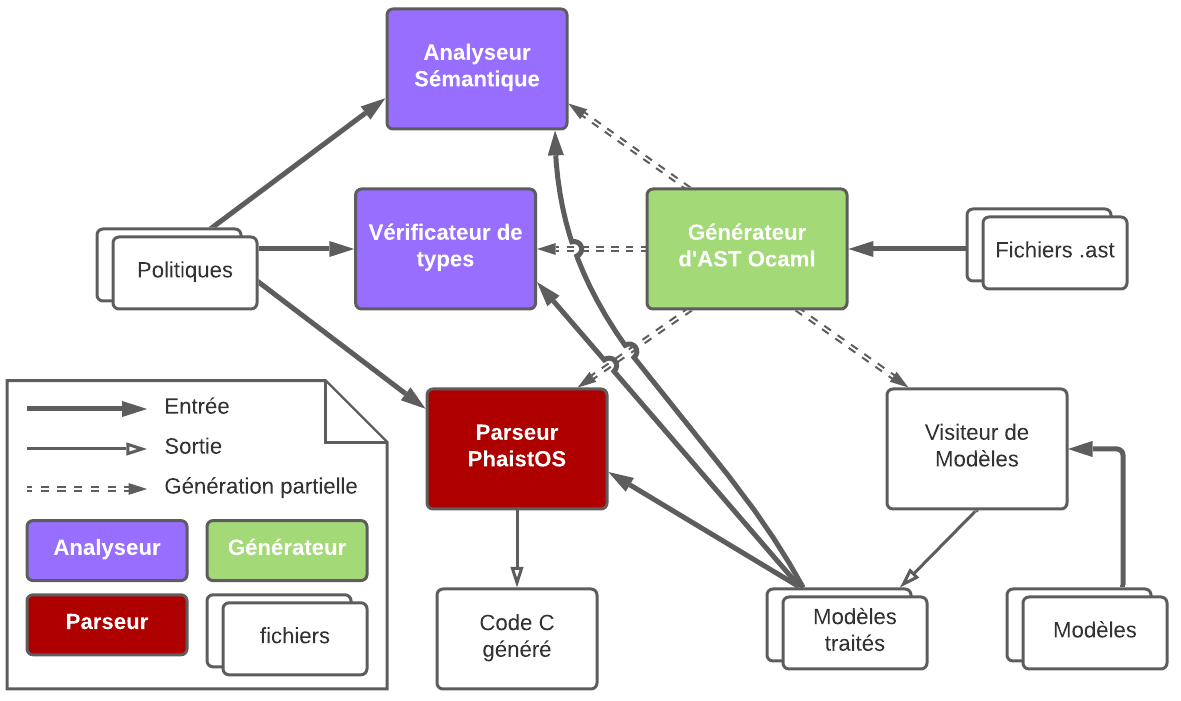
\includegraphics[width=\textwidth]{images/compiler}
    \caption{Schéma de fonctionnement du compilateur.}
    \label{fig:compiler}
\end{figure}

On remarque sur ce schéma que certaines entités importante, comme le parseur, 
sont issus d'une génération partielle, cela signifie que certains des fichiers 
du code source utilisé par le parseur sont générés. Le générateur en question 
s'appelle ``le parseur d'arbre à syntaxe abstraite interrogeable'' (``Queryable 
AST Parser'' en anglais). Son but est de transformer une description d'AST (un 
arbre abstrait) contenu dans un fichier, en code source Ocaml pouvant modéliser 
chaque noeud de l'arbre (grace à un système d'objet propre au langage) et les 
parcourir à l'aide d'un visiteur dédié à cet arbre. Par exemple, dans le cas du 
parseur, on fournira au générateur la description d'un AST qui définit la 
structure que doit avoir les politiques écrites par les utilisateurs. Cette 
description est contenue dans le fichier \texttt{phaistos.ast}, dont un extrait 
est disponible sur la Figure~\ref{fig:policy_ast}. Comme on peut le voir dans 
l'extrait à la Ligne~\ref{script_rule}, on retrouve la racine de l'arbre 
appelée \texttt{script}, le point d'entré qui va contenir toutes les 
déclarations de haut niveau d'une politique PhaistOS dans la variable \texttt
{topLevelStmts}. Comme préséntés dans la Partie~\ref{phlang}, on retrouve dans 
ces déclarations les définitions globales, l'état de la politique et la liste 
d'événements (Ligne~\ref{globdef}, Ligne~\ref{policydef} et Ligne~\ref
{eventlist} respectivement).

\begin{figure}[h!t] \centering
    \begin{tabular}{c}
        \begin{lstlisting}[language=Phaistos-AST, linewidth=13.5cm]
script (topLevelStmts: topLevel list)(*\label{script_rule}*)
topLevel () >
    | globalDefinition (var: varDecl, initExpr: expression) (*\label{globdef}*)
    | policyDeclaration (vars: varDecl list)(*\label{policydef}*)
    ...
    | eventDeclaration (events: event list)(*\label{eventlist}*)
    ...
event (name: string, typeName: string option,
       vars: varDecl list)
...
        \end{lstlisting}
    \end{tabular}
    \caption{Extrait du fichier \texttt{phaistos.ast}.}
    \label{fig:policy_ast}
\end{figure}

Concrétement, le code Ocaml du générateur prend un fichier \texttt{.ast} en 
entrée et utilise les bibliothèques Menhir et Ocamllex pour parser son contenu. 
Il va ensuite générer une sortie sous forme de code source Ocaml qui contiendra 
une classe pour chaque noeud de l'AST (voir Figure~\ref{fig:equivalent_script})
. Le code contiendra aussi une classe d'objet \textbf{visiteur} avec une 
méthode \texttt{visit} pour chaque type de noeud, comme à la Ligne~\ref
{visitcall} où le noeud \texttt{script} accepte le visiteur en appellant la 
méthode \texttt{visit\_script}.

\begin{figure}[h!t] \centering
    \begin{tabular}{c}
        \begin{lstlisting}[language=Phaistos-AST, linewidth=15cm]
script (topLevelStmts: topLevel list) = 
  object(self)
    inherit astNode as super
    val mutable topLevelStmts = topLevelStmts
    // -- snip --
    method accept visitor = visitor#visit_script (self :> script)(*\label{visitcall}*)        
end
        \end{lstlisting}
    \end{tabular}
    \caption{Équivalent Ocaml du noeud \texttt{script}.}
    \label{fig:equivalent_script}
\end{figure}

Cette visite de noeud est importante car elle permettra au parseur par la suite d'effectué une action particulière pour chaque noeud de l'arbre. 

<présenter les templates>

\subsubsection{Vérification statique}

En réalité, comme on le voit sur la Figure \ref{fig:arch}, il existe trois 
analyseurs : 
\begin{enumerate}
    \item Un analyseur sémantique de base, contenu dans \texttt{Static-Analysis}
    , écrit en Ocaml. Il permettra de vérifier l'arborescence et la sémantique 
    de la politique de l'utilisateur final. Pour cela il vérifie des règles de 
    bases, comme le parenthésage ou la présence de certains champs obligatoires.
    \item Un analyseur de type contenu dans \texttt{TypeSystem}, écrit en OCaml 
    et qui vient compléter l'analyseur précédent. Il vérifiera que les types 
    utilisés dans la politique écrite par l'utilisateur final sont corrects.
    \item Un vérificateur de propriétés de sécurité dans \texttt
    {Linear-Logic-Analysis}, concernant l'utilisation de l'API des requêtes d'E/
    S de Linux, à l'aide d'un outil externe, Celf~\cite{schack2008celf}.
\end{enumerate}
Mon stage n'a pas porté sur les analyseurs statiques, cependant les analyseurs 
écrits en Ocaml se rapproche de par leurs fonctionnement, au reste du DSL, j'ai 
donc pu travailler certains de leurs aspects.

% Pour comprendre le fonctionnement des analyseurs écrits en Ocaml, il faut 
% d'abord comprendre celui du DSL de manière générale.

\subsubsection{PhaistOS dans Linux}

<présenter son implémentation dans linux A MON ARRIVEE>

\subsection{Et ensuite ?}

<revenir sur les choses non-réalisées/complétées>

% L'analyseur en question est en réalité séparé en deux parties : une partie qui s'occupe de la vérifications des types et une autre pour exercer des vérifications spécifiques au domaine, qui utilise un système de preuve par logique linéaire.